%\title{גיאומטריה חישובית}
\documentclass{article}
\usepackage{graphicx}
\usepackage[utf8x]{inputenc}
\usepackage[english,hebrew]{babel}
\selectlanguage{hebrew}
\usepackage[normalem]{ulem}
\usepackage[top=2cm,bottom=2cm,left=2.5cm,right=2cm]{geometry}
\usepackage[fleqn]{amsmath}
\usepackage{amsthm}
\usepackage{graphicx,wrapfig,lipsum}
\usepackage{color,soul}
 \usepackage{authblk}
\usepackage{indentfirst}
\usepackage{mathtools}
\usepackage{amsfonts, amsthm, amssymb, amsmath, cancel, comment}
\usepackage{siunitx}
\usepackage{bidihl}
\usepackage[shortlabels]{enumitem}

\usepackage{amsmath,amssymb,amsthm,mathrsfs,amsfonts,dsfont}
\newtheorem{theorem}{Theorem}
\newtheorem{lemma}[theorem]{Lemma}
\newtheorem{corollary}[theorem]{Corollary}
\newtheorem{claim}[theorem]{Claim}
\newtheorem{conjecture}[theorem]{Conjecture}
\newtheorem{fact}[theorem]{Fact}
\newtheorem{definition}[theorem]{Definition}
\newtheorem{property}[theorem]{Property}

\DeclarePairedDelimiter\ceil{\lceil}{\rceil}
\DeclarePairedDelimiter\floor{\lfloor}{\rfloor}
\newenvironment{spmatrix}[1]
 {\def\mysubscript{#1}\mathop\bgroup\begin{pmatrix}}
 {\end{pmatrix}\egroup_{\textstyle\mathstrut\mysubscript}}
 
\usepackage{accents}

\newcommand{\uwidehat}[1]{%
  \mathpalette\douwidehat{#1}%
}

\newcommand{\uhat}{\underaccent{\check}}

\makeatletter
\newcommand{\douwidehat}[2]{%
  \sbox0{$\m@th#1\widehat{\hphantom{#2}}$}%
  \sbox2{$\m@th#1x$}
  \sbox4{$\m@th#1#2$}
  \dimen0=\ht0
  \advance\dimen0 -.8\ht2
  \dimen2=\dp4
  \rlap{%
    \raisebox{\dimexpr\dimen0-\dimen2}{%
      \scalebox{1}[-1]{\box0}%
    }%
  }%
  {#2}%
}
\makeatother

\usepackage{titlesec, url, color}

\setcounter{secnumdepth}{4}
\def\titlefootnote{\ifx\protect\@typeset@protect\expandafter\footnote\else\expandafter\@gobble\fi}
\makeatletter
\def\@xfootnote[#1]{\protected@xdef\@thefnmark{#1}\@footnotemark\@footnotetext}
\newcommand\abs[1]{\left|#1\right|}

\makeatletter
\titleformat{\paragraph}
{\normalfont\normalsize\bfseries}{\theparagraph}{1em}{}
\titlespacing*{\paragraph}
{0pt}{3.25ex plus 1ex minus .2ex}{1.5ex plus .2ex}

\setcounter{secnumdepth}{5}

\titleformat{\subparagraph}
{\normalfont\normalsize\bfseries}{\thesubparagraph}{1em}{}
\titlespacing*{\subparagraph}
{0pt}{3.25ex plus 1ex minus .2ex}{1.5ex plus .2ex}


\makeatletter
\newcommand*{\saved@uline}{}
\let\saved@uline\uline

\newcommand*{\mathuline}{%
  \mathpalette{\math@uline\saved@uline}%
}
\newcommand*{\math@uline}[3]{%
  % #1: ulem command
  % #2: math style
  % #3: contents
  \mbox{#1{$#2#3\m@th$}}%
}

% optional
\renewcommand*{\uline}{%
  \relax  
  \ifmmode
    \expandafter\mathuline
  \else
    \expandafter\saved@uline
  \fi
}


\title{ גיאומטריה חישובית }
\selectlanguage{english}

\author{lages dalig}
\selectlanguage{hebrew}


\begin{document}
\maketitle


\section{ פעולות אטומיות}
\noindent אוסף של פעולות שניתן לבצע במספר קבוע של מהלכים

\subsection{נקודות בשתי צדי ישר}
\noindent \uline{קלט:} שתי נקודות $p,q$ וישר $L$
\newline \uline{ שאלה:} האם $p,q$ נמצאים באותו צד של הישר $L$
\newline \uline{פתרון:} נציב את הנקודות על משוואת הישר ונבדוק האם יש להן את אותו הסימון

\subsection{שיוך נקודה לקטע}
\noindent \uline{קלט:} קטע $pq$ ונקודה $w$
\newline \uline{ שאלה:} האם הנקודה $w$ נמצאת על הקטע
\newline \uline{פתרון:} 1. נבדוק האם הנקודה על הישר 2. נבדוק האם ערך ה$X$ של $w$ נמצא בין ערכי ה$X$ של $p$ ושל $q$ )אם הקטע אנכי לצירים נבדוק על $Y$(

\subsection{זיהוי כיוון של ווקטורים}
\noindent \uline{קלט:} $p_0p_1$ , $p_0p_2$ וקטורים
\newline \uline{שאלה:} האם $p_0p_1$ בכיוון השעון כלפי $p_0p_2$ )שאלה זהה האם הזויות בינהם מתחת ל$\ang{180}$(
\newline \uline{פתרון:} ננרמל את הווקטרים לראשית הצירים ונחשב את המכפלה הקרטזית אם קיבלנו מספר חיובי הזויות מתחת ל$\ang{180}$

\subsection{זיהוי כיוון פנייה}
\noindent \uline{קלט:} $p_0p_1$ , $p_1p_2$ וקטורים
\newline \uline{שאלה:} האם $p_1p_2$ פונה ימינה מ $p_0p_1$
\newline \uline{פתרון:} נהפוך את הווקטר $p_0p_1$ ונקבל את אותה השאלה כמו סעיף קודם

\subsection{נקודות בציר ישר}
\noindent \uline{קלט:} $p_1$ $p_2$ נקודות $l_3l_4$ ישר
\newline \uline{שאלה:} האם הנקודות $p_1$ $p_2$ נמצאות באותו צד של הישר 
\newline \uline{פתרון א':} שימוש בפעולה אטומית 1.1
\newline \uline{פתרון ב':} שימוש בפעולה אטומית $1.4$ נבדוק את הכיוון של הווקטור $l_4p_2$ ביחס ליישר ואת הכיוון של הווקטור $l_4p_1$ ביחס ליישר, אם זה אותו כיוון אז הם באותו צד

\subsection{חיתוך קטעים}
\noindent \uline{קלט:} $p_1p2$ $p_3p_4$ שני קטעים
\newline \uline{שאלה:} האם הקטעים נחתכים
\newline \uline{פתרון:} ניקח את הווקטור  $p_1p_2$ ונבנה את משוואת הישר שלו ונבדוק מה הצד של שני הנקודות $p_3$ ו$p_4$ נעשה את אותו הדבר עם הישר $p_3p_4$ )צריך גם וגם( 
\newline \uline{מקרה קצה:} אם הישרים נמצאים על אותו הישר 



\subsection{אורך קטע}
\noindent \uline{קלט:} $p_1p_2$  קטע
\newline \uline{שאלה:} אורך הקטע
\newline \uline{פתרון:} $d= \sqrt{(p_{1_x}-p_{2_x})^2+(p_{1_y}-p_{2_y})^2}$ 

\subsection{מרחק נקודה מישר}
\noindent \uline{קלט:} $p_1p2$  ישר $q$ נקודה
\newline \uline{שאלה:} מרחק הנקודה מהישר
\newline \uline{פתרון:} נוריד אנך מהנקודה אל הישר ונחשב את האורך שלו  $d=\abs{\frac{a*q_x-q_y+b}{ \sqrt{a^2+1}}}$

\subsection{זויות כהה בין ווקטורים}
\noindent \uline{קלט:} $p_0p_1$ $p_0p_2$ שני ווקטורים
\newline \uline{שאלה:} האם הזווית בין הווקטרים כהה
\newline \uline{פתרון:} ננרמל את הווקטורים לראשית הצירים ונכפיל או(תם מכפלה פנימית אם התוצאה חיובית הזוויות כהה

\subsection{האם לשני קטעים יש נקודות עם קורדינטת $X$ משותפת )כאשר ערך ה$Y$ לא משנה(}
\noindent \uline{קלט:} שני קטעים
\newline \uline{שאלה:} האם יש להם קורדינטת $X$ משותפת 
\newline\uline{פתרון}
\subsection{מציאת נקודה פנימית במשולש}
\noindent \uline{קלט:} $\triangle p_1p_2p_3$ משולש
\newline \uline{שאלה:} מצא נקודה הנמצאת בתוך המשולש )לא על השפה(
\newline \uline{פתרון:}  קורדינטת $X$ תהיה $(p_{1_x}+p_{2_x}+2p_{3_x})/4$ קורדינטת $Y$ תהיה $(p_{1_y}+p_{2_y}+2p_{3_y})/4$

\subsection{האם נקודה בתוך משולש}
\noindent \uline{קלט:} $\triangle p_1p_2p_3$ משולש $q$ נקודה
\newline \uline{שאלה:} האם הנקודה $q$ נמצאת בתוך המשולש )או על השפה(
\newline \uline{פתרון:} נמצא נקודה במשולש $w$ )באמצעות הסעיף הקודם( נבדוק האם הנקודה $q$ נמצא באותו צד כמו הנקודה $w$ כלפי כל אחד מהישרים של המשולש 

\section{ סגור קמור}
ניתן לחשוב על הקמור כעל גומייה שנמתחה כך שתקיף את כל הנקודות/ המסמרים, ולאחר מכן שוחררה.\\
\selectlanguage{english}
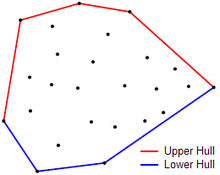
\includegraphics[scale=0.7]{z1.png}
\selectlanguage{hebrew}

\noindent\uline{קבוצה קמורה:} הקבוצה $S$ תקרא קבוצה קמורה אם לכל $p,q\in S$ הקטע שמחבר בין הנקודות $pq\in S$
\newline\newline\textbf{למה} חיתוך שני קבוצות קמורות נותן קבוצה קמורה
) נוכיח בשלילה שקיים $q,p\in S$ כך שהקטע $qp$ לא נמצא בחיתוך $S\cap S'$ \textbf{אבל} לפי ההגדרה $pq \in S$ וגם $pq \in S'$ (

\subsection{הגדרות}
\uline{מצולע}
\begin{enumerate}
\item $P_v$ קדקודי המצולע
\item $P_e$ צלעות המצולע
\item $P_a$ שטח המצולע
\end{enumerate}
\uline{עקום} קו מפותל
\newline\uline{עקום סגור} סדרה של קטעים סגורים
\newline\uline{עקום פשוט} עקום כך שאף שתי צלעות לא נחתכות
\uline{מצולע קמור}
\begin{itemize}
\item מצולע פשוט וסגור שהשטח $P_a$ חוסם קבוצה קמורה
\item מצולע פשוט וסגור כל הזויות הפנימיות שלו קטנות מ$\ang{180}$
\end{itemize}

\uline{ סגור קמור )סימון $CH$(}
\begin{itemize}
\item בהינתן קבוצת קדקודים $S$ נגדיר את $CH(S)$ להיות הקבוצה הקטנה ביותר המכילה את $S$
\item $CH(S)$ יהיה חיתוך של כל הקבוצות המכילות את $S$
\end{itemize}


\subsection{אלגוריתמים נאייבים לחישוב סגור קמור}
בהינתן קבוצת נקודות $S$ נדרש אלגוריתם שימצא לנו את $CH(S)$
\subsubsection{הנחות}
\begin{enumerate}
\item $p$ לא יהיה קדקוד ב$P_v$ \textbf{אם ורק אם}
\begin{itemize}
\item קיים $p_i,p_j \in S$ כך ש$p$ נמצא על הישר $p_ip_j$
\item )או( קיים $p_i,p_j,p_k \in S$ כך ש$p$ נמצא במשולש $\triangle p_ip_jp_k$
\end{itemize}
\item $pq$ תהיה צלע ב $P$ אם ורק אם  $\forall w \in S$ הנקודה $w$ נמצאת על אותו צד של הישר $pq$ 
\end{enumerate}

\subsubsection{אלגוריתמים נאיבים}
\begin{enumerate}
\item נעבור על כל הנקודות ב$S$ ונבדוק האם הן שייכות ל$P_v$ $\leftarrow$ זמן ריצה $\mathcal{O}(n^4)$ \textbf{האלגוריתם לא מחזיר את סדר הצלעות}
\item נעבור על כל זוגות הנקודות ב$S$ ונבדוק האם הן צלע $\leftarrow$ זמן ריצה $\mathcal{O}(n^3)$
\item ניקח את הנקודה $p_0$ הכי שמאלית עם $X,Y$ מינימלי )בהכרח קדקוד( נמצא ל$p_0$ את הצלע שלה $p_1$ ול$p_1$ נמצא את הצלע שלה $p_2$ עד שנגיע ל$p_h$ $\leftarrow$ זמן ריצה $\mathcal{O}(n^2*h)$ 
\end{enumerate}


\subsection{אלגוריתם סריקת גרהם}
\begin{itemize}
\item מיין את הנקודות לפי קורדינטות  $x$ כך ש: $x_1 < x_2 < \cdots < x_n$
\item נסרוק את הנקודות משמאל לימין. אחרי $i$ איטרציות, חישבנו את $\hat{CH_i}= \hat{CH}(p_1, \cdots, p_i)$
\end{itemize}
\uline{הבחנה:} לאוסף נקודות $S=\{\ell_1, \cdots, \ell_n \}$ הקמור העליון $\hat{CH}(S)$ הוא אוסף נקודות $Q$ שיוצר שרשרת צלעות עם התכונות הבאות:
\begin{enumerate}
\item $Q_i$ מתחיל ב- $p_1$ ומסתיים ב-$p_i$
\item השרשרת נמצאת מעל כל הנקודות של $S_i$
\item בטיול על שרשרת מ- $p_1$ ל-$p_i$, כל הפניות הן פניות ימינה
\end{enumerate}
מחסנית $\mathcal{S}$ מחזיקה את נקודות הקמור העליון $Q_i$ לפי סדרן.\\ $p_{top}$- הנקודה שנמצאת בראש המחסנית, $p_{2nd}$- הנקודה שנמצאת במחסנית מתחת ל-$p_{top}$\\
\uline{איתחול:} $push(p_1), push(p_2)$\\
\uline{לכל $i$ מ-3 עד $n$ בצע:}
\begin{itemize}
\item 
כל עוד יש במחסנית לפחות 2 נקודות, ושלש הנקודות $p_{2nd}, p_{top}, p_i$ מהוות פניה שמאלה, בצע $pop$
\item בצע $push(p_i)$
\end{itemize}
\uline{טענת נכונות:} לאחר איטרציה $i$, תכולת המחסנית מהווה את $\hat{CH}(S_i)$\\
\uline{סיבוכיות:} $\mathcal{O}(n \log(n))$ )המיון. הערה: כל השאר $\mathcal{O}(n)$(\\
\paragraph{הערות }
\begin{enumerate}
\item ייתכן והקמור העליון לא ייפגש עם הקמור התחתון )במידה ולשתי הקצוות אותו ערך של $X$ במידה וכן נחבר בין הנקודות(
\item ניתן לבצע את האלגוריתם בפעם אחת ללא קמור עליון ותחתון על ידי מיון פולארי של הנקודות ולרוץ מנקודה אחת עם כיוון השעון
\end{enumerate}


\paragraph{בעיית הגלריה }
למצוא מספר מינימלי של נקודות מהן אפשר לראות את כל המצולע.\\
במצולע קמור מספיקה נקודה אחת.\\
במצולע קעור: ישנן צורות בהן מספיקה נקודה אחת, למשל: \L{star-shaped polygon}\\
\selectlanguage{english}
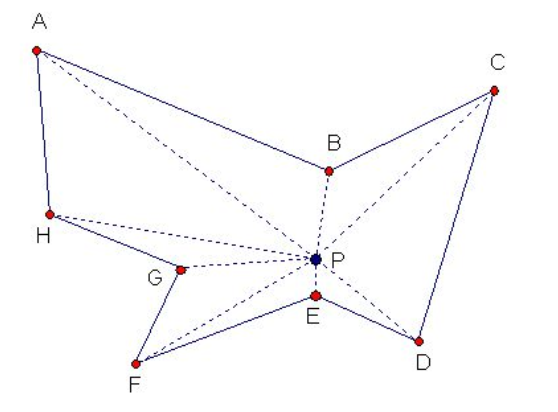
\includegraphics[scale=0.3]{z3.png}
\selectlanguage{hebrew}
\\
אך יתכן שידרשו יותר נקודות:\\
\selectlanguage{english}
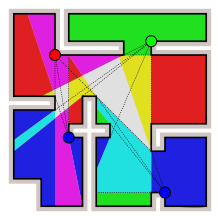
\includegraphics[scale=0.3]{z2.png}
\selectlanguage{hebrew}\\
במצולע דמוי כוכב אפשר לחשב את הסגור הקמור בלי המיון.\\


\noindent\textbf{תרגיל:} נניח שאוסף הנקודות $S$ נבחר באקראי בריבוע היחידה. מה ניתן לומר על תוחלת הסיבוכיות של אלגוריתם גרהם?


\subsection{אלגוריתם עטיפת המתנות}
\begin{enumerate}
\item מצא את הנקודה הנמוכה ביותר ב-$S$, $p_0$ $(\mathcal{O}(n))$
\item השווה את הנקודות על פי הזווית של $p_0 p_i$ ביחס לקרן ימינה מ-$p_0$, ובחר את $p_1$ בעלת הזווית הקטנה ביותר
\item לכל $i \geq 1:$ לאחר מציאת $p_i$: חפש את $p_{i+1}$ בעלת הזווית הקטנה ביותר בין $\overrightarrow{p_i p_{i+1}}$ לקרן מ-$p_i$ ימינה $(\mathcal{O}(n))$
\end{enumerate}
$\uhat{CH}(S)= <q_1m \cdots, q_h>$\\
$h=|\uhat{CH}(S)|$\\
סיבוכיות כוללת: $\mathcal{O}(n \cdot h)$\\
\uline{שאלה:} מהי תוחלת $|\uhat{CH}(S)|$ כש-$S$ נבחרה באקראי בריבוע היחידה?\\
\uline{תשובה:} $E(h)= \mathcal{O}(\log(n))$\\
\uline{טענה:} $E(|C_{UR}|)= \mathcal{O}(\log(n))$\\
\uline{הגדרה:} הנקודה $p=(x,y)$ שולטת על הנקודה $p'=(x',y')$ אם $x \geq x'$ ו-$y \geq y'$.\\
נקודה ב-$S$ נקראת בלתי נשלטת אם אף נקודה אחרת ב-$S$ לא שולטת עליה.\\
$B$= קבוצת הנקודות הבלתי-נשלטות מ-$S$ ברביע הראשון.\\
$C_{UR} \subseteq B$\\
\uline{טענה:} $E(|B|)= \mathcal{O}(\log(n))$\\
\uline{נימוק:} נמיין את נקודות $S$ בסדר $X$ לא עולה $x_1 \geq \cdots \geq x_n$\\
\uline{הבחנה:}
$p_i=(x_i, y_i)$ לא שלטת אם"ם $y_i$ היא המקסימלית מבין $p_1, \cdots, p_i$ )כלומר, $y_i>y_1, y_2, \cdots, y_{i-1}$(\\
$\Pr(y_i>y_1, y_2, \cdots, y_{i-1})= \frac{1}{i}$\\
$E(|B|)= \sum_{i=1}^n \frac{1}{i}= \mathcal{O}(n)$\\
\textbf{תרגיל 1:} בהינתן אוסף $S$ של $n$ נקודות, מצא את כל הנקודות הלא נשלטות ב-$S$. )קל: $\mathcal{O}(n^2)$. למצוא יותר יעיל: $\mathcal{O}(n \log(n))$(\\


\subsection{חסם תחתון}
\noindent\uline{משפט:} חישוב הסגור הקמור של $n$ נקודות במישור )מוחזר על פי סדר הקודקודים על הסגור( דורש $\Omega(n \log(n))$ פעולות במקרה הגרוע במודל הפעולות האלגבריות.\\
\uline{הוכחה:} נסתמך על כך שמיון דורש $\Omega(n \log(n))$ פעולות במקרה הגרוע.\\
נניח שיש לנו פרוצדורה $A$ לחישוב סגור קמור, נראה אלגוריתם מיון בסיבוכיות $T_A+\mathcal{O}(n)$\\
\textbf{אלגוריתם למיון:}
\uline{קלט:} $x_1, \cdots, x_n$ טבעיים שונים\\
\begin{enumerate}
\item ניצור קלט לבעיית $CH$: $S=\{ p_1=(x_1, x_1^2), c\dots, p_n=(x_n, x_n^2) \}$
\item נפעיל את $A$ ונקבל מצולע $P=CH(S)= <q_1, q_2, \cdots, q_n>$\\
\selectlanguage{english}
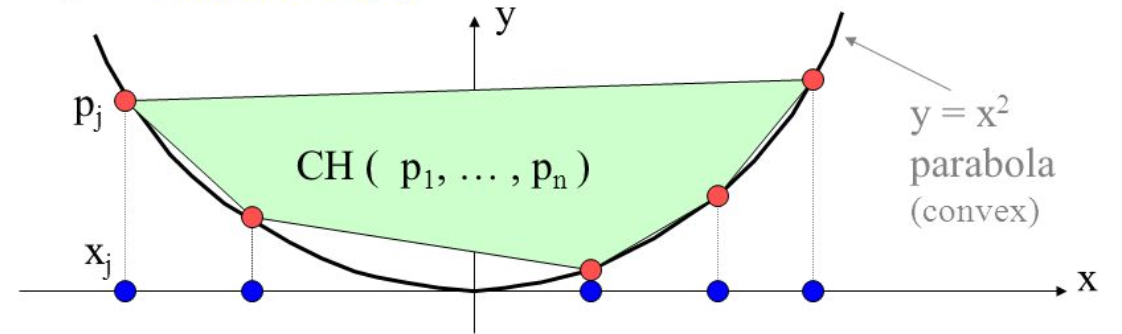
\includegraphics[scale=0.2]{z4.png}
\selectlanguage{hebrew}\\
\item מתוך $P$ נחלץ את הסדרה הממוינת.
\end{enumerate}

\subsection{אלגוריתם מיזוג קמורים}
\begin{enumerate}
\item אם גודל הקבוצה $S$ שווה 3 החזר את $S$
\item חלק את $S$ לשתי קבוצות זרות בגודל שווה ועבור כל קבוצה תפעיל את האלגוריתם
\item מזג בין שני הסוגרים הקמורים שהתקבלו
\end{enumerate}

\paragraph{אלגוריתם עזר "מיזוג קמורים"  $S',S$}
\begin{enumerate}
\item נקח את הקמור העליון של $S$ ושל $S'$ ונמזג אותם על ידי האלגוריתם של גרהם )רק שעכשיו שתי הקבוצות ממוינות כבר( כנ"ל לקמור התחתון
\item אחד בין הקמור התחתון לקמור העליון
\end{enumerate}
\noindent\uline{סיבוכיות} $\mathcal{O}(n\log(n))$ )מתאים לעיבוד מקבלי(
\noindent\textbf{תרגיל:} נניח שאוסף הנקודות $S$ נבחר באקראי בריבוע היחידה. מה ניתן לומר על תוחלת הסיבוכיות של האלגוריתם?

\subsection{אלגוריתם קירקפטריק}

\paragraph{מבנה נתונים היררכי}
$H_{i+1}$ יכיל כל קדקוד שני מהמצולע $H_i$ כאשר $H_0=CH(S)$ 
\selectlanguage{english}
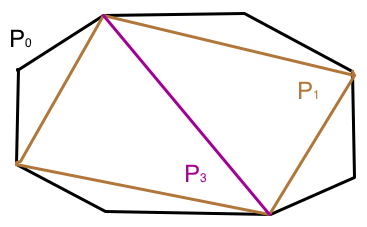
\includegraphics[scale=0.4]{z5.png}
\selectlanguage{hebrew}\\

\paragraph{שאילתת קיצון}
\noindent\uline{קלט} $q$ נקודה חיצונית לסגור הקמור וישר $L$ שעובר דרך הנקודה  
\newline\uline{שאלה} אם נסובב את הישר $L$ על הציר של $q$ באיזו נקודה מ$S$ אני אפגע ראשונה )ניתן לשים לב שכל נקודה פנימית בתוך הסגור לא יכולה להתקבל כפתרון(
\newline\uline{פתרון} נבנה עבור $CH(S)$ מבנה נתונים היררכי $H$ 
\begin{enumerate}
\item עבור $H_k$ נבצע את הפעולה האטומית האם הנקודה נמצאת על הישר
\item עבור $H_{i-1}$ הנקודה חייבת להיות 
\begin{itemize}
\item קדקוד ברמה $H_i$
\item אחד מהשכנים הצמודים של המצולע $H_i$
\end{itemize}
\end{enumerate}

\noindent\textbf{תיאור האלגוריתם )בהנחה וכמות הקדקודים $h$ ידועה מראש( }
\begin{enumerate}
\item חלק את הנקודות ל$k=\frac{n}{h}$ קבוצות $\leftarrow$ $\mathcal{O}(n)$
\item לכל קבוצה חשב את הסגור הקמור ושמור אותה במבנה נתונים היררכי $\leftarrow$ $\mathcal{O}(n\log(h))$
\item בצע את אלגוריתם עטיפת המתנות באופן הבא
\begin{itemize}
\item מצא את הנקודה $p_0$ השמאלית הנמוכה ביותר $\leftarrow$ $\mathcal{O}(n)$
\item עבור כל קבוצה נבצע על הנקודה $p_0$ את שאילתת הקיצון שלנו )נקבל סך הכל k מועמדים( מבין המועמדים נבחר את האחד עם הזוויות הנמוכה ביותר כלפי $p_0$ )מזכיר את אלגוריתם עטיפת המתנות אך חוסך לנו את המיון( $\leftarrow$ $\mathcal{O}(h*[k+k\log(h)])=\mathcal{O}(n\log(h))$
\end{itemize}
\end{enumerate}

\noindent\uline{סיבוכיות}  אם נשערך את $h \in [1,2,4,8,16....,2^i]$ עד שנקבל את התוצאה $\mathcal{O}(n\log(h)* \log(h))$ אם נשערך את $h \in [4,16,256,....,2^{2^i}]$ עד שנקבל את התוצאה $\mathcal{O}(n\log(h))$ 

\subsection{סגור קמור אונלין}
\noindent\uline{הגדרה} בהינתן סגור קמור $S$ ונקודה $p_{n+1}$ הוסף את הנקודה כך ש$CH(S_{n+1})=CH(S \cup p_{n+1})$
\paragraph{הגדרות}
\selectlanguage{english}
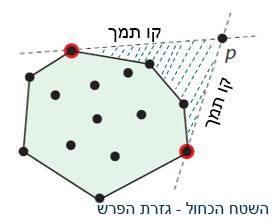
\includegraphics[scale=0.7]{z6.png}
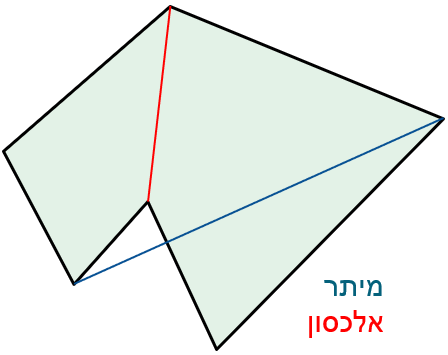
\includegraphics[scale=0.4]{z7.png}
\selectlanguage{hebrew}\\
\begin{enumerate}
\item \uline{תת מצולע קמור} נגדיר מצולע $P$ ואת המצולע $P'$ תת מצולע קמור של $P$ אם $P'$ מכיל חלק מהקדקודים של $P$
\item \uline{קו תמך} בהינתן מצולע קמור $S$ ונקודה $p$ נעביר קרן עם כיון השעון מהנקודה $p$ נעצור בנקודת החיתוך הראשונה עם המצולע $S$ לקו שנוצר נקרא קו תמך )כנ"ל נעביר קרן נגד כיוון השעון(
\item \uline{שרשרת על המצולע} בהינתן שתי נקודות $p,q$ על השפה של המצולע $S$ נגדיר את השרשת להיות השפה של המצולע בין $p,q$ )כאשר בפועל מקבלים שתי שרשראות(
\item \uline{מיתר} הקטע  $p_ip_j$ כש $p_i$ ו$p_j$ הם קדקודים לא סמוכים של המצולע
\item \uline{מיתר מתחלף} מיתר $A$ מתחלף עם המיתר $B$ אם אחד הקצוות של $B$ נמצא בשרשרת אחת של $A$ והקצה השני נמצא בשרשרת השנייה של $A$
\item \uline{אלכסון} מיתר המוכל כולו בתוך המצולע
\item \uline{גזרת הפרש} המצולע המתקבל בין הנקודה החיצונית לבין המצולע $S$ 
\end{enumerate}

\paragraph{הבחנות}
\begin{enumerate}
\item במצולע קמור כל שני מיתרים מתחלפים בהכרח נחתכים )וגם להפך אם הם נחתכים הם מתחלפים( \textbf{)תרגיל הוכח(}
\item $S$ מצולע קמור, $S'$ תת מצולע קמור של $S$ ונקודה $q$ חיצונית ל$S'$ גזרת ההפרש של $q$ איחוד $S'$ מהווה מצולע קמור \textbf{)תרגיל הוכח(} 
\end{enumerate}

\textbf{אלגוריתם דינאמי למציאת סגור קמור}
\begin{enumerate}
\item הרץ שאילתת קיצון מוכללת על $p_{n+1}$ אם הנקודה לא פנימית בצע איחוד בין $C_{far}$ \footnote{השרשת הרחוקה מנקודות התמך} לבין גזרת ההפרש בצע תיקון למבנה הנתונים ההיררכי
\end{enumerate}
\uline{סיבוכיות} $\mathcal{O}(\log(n))$

\textbf{הערות}
\begin{itemize}
\item עבור מבנה נתונים הררכי $H$ נגדיר "קשת מסכנה" להיות קשת של $H_i$ שמופיעה ב$H_{i+1}$ )במצב תקין מותר עד קשת מסכנה אחת בכל $H_i$(
\item בעת התיקון של מבנה הנתונים ההיררכי נקבל מצב שבתיקון מתקבל שתי קשתות מסכנות סמוכות על מנת לתקן נאחד 
\end{itemize}


\section{חיתוכי קטעים}
\subsection{הקדמה}
\selectlanguage{english}
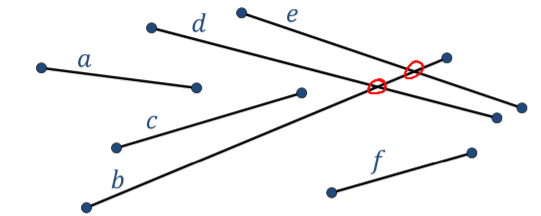
\includegraphics[scale=0.8]{z8.png}
\selectlanguage{hebrew}

הגדרה : נתון $S$ קבוצות כך שכל קבוצה מכילה $n$ קטעים 
\begin{enumerate}
\item \uline{בעיית החלטה} האם יש זוג קטעים שנחתך )אלגוריתם נאיבי $\mathcal{O}{n^2}$ (
\item \uline{בעיית מציאה} מצא את כל זוגות הקטעים שנחתכים )כאשר במקרה הגרוע יהיה $O(n^2)$ קטעים(
\end{enumerate}
\noindent\uline{המקרה החד מימדי} אנחנו נמצאים על ציר $X$
\newline\uline{פתרון} כל קטע $q$ נגדיר בתור $(q_l,q_r)$ נמיין את הנקודות אם קיבלנו פעמיים ברצף $r$ אז וערכי ה$X$ שלו שונים אז יש חיתוך
\newline\uline{חסם תחתון למקרה הכללי} $\mathcal{O}(n\log(n))$ הוכחה באמצעות רדוקציה מבעיית יחידות אלמנטים (בהינתן קבוצה של $n$ אלמנטים לקבוע האם יש מספר שמופיע יותר מפעם אחת(
\subsection{אלגוריתם קו הסריקה}
\selectlanguage{english}
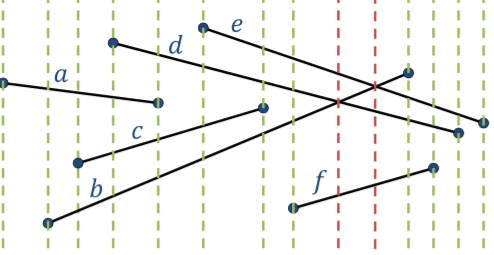
\includegraphics[scale=0.75]{z9.png}
\selectlanguage{hebrew}

\uline{הנחות מפשטות}
\begin{enumerate}
\item אין קטעים אנכיים \footnote{כאשר לא מריצים את סעיף ג' באלגוריתם}
\item כל נקודת חיתוך היא של מקסימום 2 קטעים
\item אין נגיעה בין נקודת קצה של קטע לקטע אחר
\item הקווים אינם משיקים זה לזה
\end{enumerate}
\subsubsection{תיאור מבנה הנתונים}
\noindent לצורך האלגוריתם נתחזק מבנה נתונים שמסגול לבצע
\begin{enumerate}
\item שומר את אוסף הקטעים הפעילים כרגע
\item מערך של $2n$ נקודות של נקודות ההתחלה והסיום של כל קטע ממוין לפי קודרינטאת $X$
\end{enumerate}
\uline{פעולות על מבנה הנתונים}  
\begin{enumerate}
\item\uline{tresni} הוספה של קטע 
\item\uline{eteled} מחיקה של קטע 
\item\uline{evoba} מציאה של הקטע מעל עם אותה קורדינאטת $X$ $\Leftarrow$ $\mathcal{O}(\log n)$ 
\item\uline{woleb} מציאה של הקטע מתחת עם אותה קורדינאטת $X$ $\Leftarrow$ $\mathcal{O}(\log n)$
\end{enumerate}
\subsubsection{תיאור האלגוריתם} 
\begin{enumerate}[label=\textbf{\arabic*}.]
\item $E\Leftarrow\emptyset$ ,$SL\Leftarrow\emptyset$
\item הכנס אל  $E$ את נקדות התחלה וסיום של הקטעים באופן ממוין
\item לכל $e \in E$ בצע:
\begin{enumerate} [)a(]
\item אם $e$ נקודת התחלה של קטע 
\begin{enumerate}
\item בצע $insert(SL,e)$ 
\item בדוק האם זוג הקטעים $(e,Above(e))$ נחתכים 
\item בדוק האם זוג הקטעים $(e,Below(e))$ נחתכים 
\end{enumerate}
\item אם $e$ נקודת סיום של קטע 
\begin{enumerate}
\item בצע $delete(SL,e)$
\item בדוק האם זוג הקטעים $(Below(e),Above(e))$ נחתכים 
\end{enumerate}
\item אם $e$ נקודת חיתוך של הקטעים $s1,s2$ 
\begin{enumerate}
\item בצע $delete(SL,s1)$, $delete(SL,s2)$
\item בצע $insert(SL,s2)$, $insert(SL,s1)$ )בסדר הפוך(
\item חסר! 
\end{enumerate}
\end{enumerate}
\end{enumerate}
\uline{סיבוכיות} המיון עולה $\mathbb{O}(n \log n)$ ומציאת החיתוכים $\mathcal{O}(k\log n)$ סך הכל $\mathcal{O}((n+k)\log n)$ כאשר $k$ מסמל את מספר החיתוכים

\noindent\uline{הערות} כאשר כל הקווים אנכיים או מקבילים לצירים אפשר להריץ את האלגוריתם בלי סעיף ג' בזמן ריצה של $\mathcal{O}(n\log n)$ 

\section{מצולעים}
\subsection{סיווג מצולעים}
\selectlanguage{english}
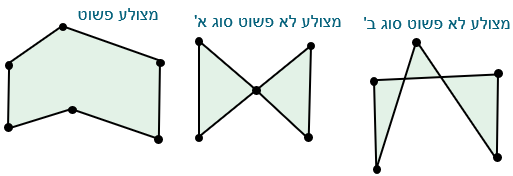
\includegraphics[scale=0.7]{z10.png}
\selectlanguage{hebrew}
\noindent\uline{בעיה} בהינתן מצולע $P$ קבע האם הוא פשוט או לא
\begin{enumerate}
\item \uline{פתרון א'} נפעיל את האלגוריתם שמוצא את החיתוכים אם יש $n$ צלעות ומצאנו $n$ חיתוכים המצולע פשוט
\item\uline{פתרון ב'} ניתן לעשות שינוי פשוט באלגוריתם של מציאת חיתוכים כך שידווח על חיתוך של אמצע של קטעים
\end{enumerate}

\subsection{ שאלות על מצולעים}
\selectlanguage{english}
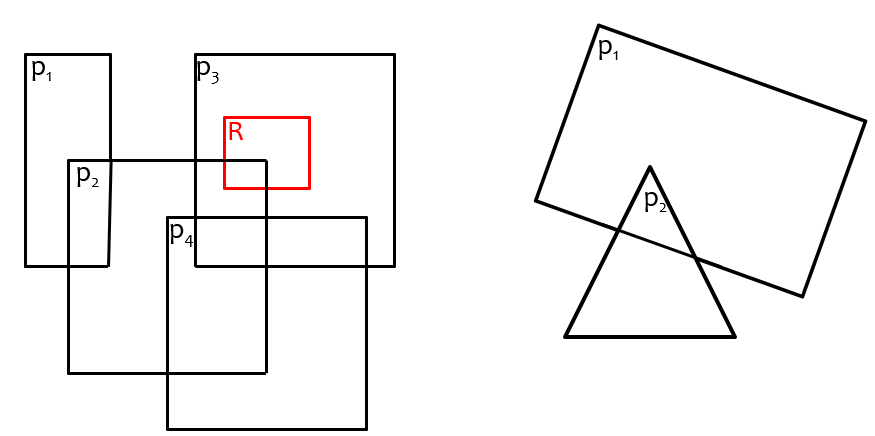
\includegraphics[scale=0.5]{z11.png}
\selectlanguage{hebrew}
\subsubsection{חיתוך מצולעים}
\noindent \uline{קלט:} מצולעים $P_1$, $P_2$
\newline \uline{ שאלה:} האם המצולעים נחתכים
\subsubsection{האם מצולע מוכל}
\noindent \uline{קלט:} מצולעים $R$, $(P_1, P_2, \cdots, P_{i-1})$
\newline \uline{ שאלה:} האם $R \subseteq \cup_{i=1}^n P_i$
\newline\uline{רמז} פתרון חמדני ב$\mathcal{O}(n^2)$

\section{חלוקת מישור}
\subsection{הקדמה}
\selectlanguage{english}
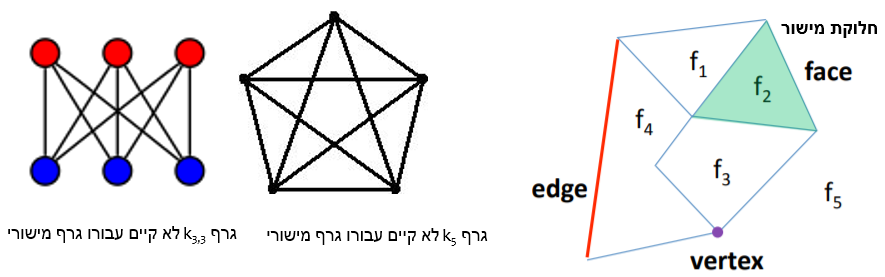
\includegraphics[scale=0.65]{z14.png} 
\selectlanguage{hebrew}
\newline\noindent\uline{גרף מישורי} גרף שניתן לשכן את הקדקודים שלו במישור כך שהצלעות שלו יהיו ללא חיתוכים )ישנם שני סוגים של גרפים להם אין גרף מישורי(
\newline\uline{חלוקת מישור} גרף מישורי שהצלעות שלו הן ישרות
\newline\uline{משפט} כל גרף מישורי ניתן לשכן אותו במישור עם צלעות ישרות )ז"א לכל גרף מישורי קיים חלוקת מישור(
\subsection{מבנה נתונים לייצוג מישור}

\selectlanguage{english}
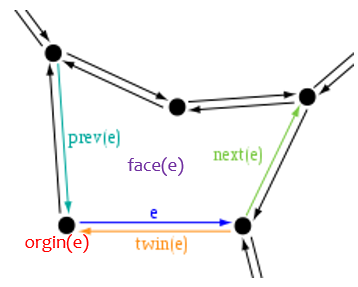
\includegraphics[scale=0.6]{z15.png} 
\selectlanguage{hebrew}


\noindent בהינתן צמתים וקשתות במישור נרצה לשמור אותם במבנה נתונים ייעיל שיאפשר לנו לבצע  פעולות מבנה נתונים זה נקרא $double-connected-edge-list$ )$DCEL$( 
\newline\noindent\textbf{הבחנות}
\begin{enumerate}
\item הגרף קשיר
\item לגרף קיים פאה חיצונית אחת בלבד
\end{enumerate}
\subsubsection{הגדרת מבנה הנתונים}
\noindent מבנה הנתונים מכיל 3 רשומות שבאמצעותן מייצגים את המישור
\begin{enumerate}
\item \uline{רשומת צומת $v$} $\Leftarrow$ $\mathcal{O}{(1)}$ \footnote{עבור הגרסה המצומת, בגרסה המקורית נקבל גודל כתלות בדרגה של הצומת}
\begin{itemize}
\item הקורדינטה של הצומת $v$
\item מצביע לרשומה של הקשתות היוצאות מהצומת )קיימת גרסה מצומצמת בה יש מצביע רק לקשת אחת, אנחנו נתייחס לייצוג המצוצם(
\end{itemize}
\item \uline{רשומת פאה $f$} $\Leftarrow$ $\mathcal{O}{(1)}$
\begin{itemize}
\item מצביע לקשת של השפה
\end{itemize}
\item \uline{רשומת קשת $e$} $\Leftarrow$ $\mathcal{O}{(\log n)}$
\begin{itemize}
\item $twin(e)$ $\Leftarrow$ מצביע לקשת התאומה  
\item $origin(e)$ $\Leftarrow$ מצביע לצומת המוצא  
\item $next(e)$ $\Leftarrow$ מצביע לקשת הבאה  
\item $prev(e)$ $\Leftarrow$ מצביע לקשת הקודמת  
\item $face(e)$ $\Leftarrow$ מבציע לפאה של הקשת  
\end{itemize}
\end{enumerate}

\subsubsection{הערות}
\begin{enumerate} 
\item \uline{משפט אוילר} $|f|=|e|-|v|+2$ כך שיש קשר בין כמות הקדקדים והקשתות  לבין כמות הפאות
\item\uline{משפט} לכל גרף מישורי עם $n\geq 4$  יש לכל היותר $3n-6$ קשתות
\item מבנה הנתונים לוקח סך הכל $\mathcal{O}(n\log n)$ בגלל שיש $\mathcal{O}(n)$ קשתות וקדקודים 
\item במקרה שהגענו במסלול לנקודת "אין מוצא" $twin(e)=next(e)$ )למשל במבנה של כוכב(
\end{enumerate}
\subsubsection{פעולות על מבנה הנתונים}
\begin{itemize}
\item טיול לאורך הגבול הפנימי של פאה
\item טיול על הקשתות היוצאות מצומת נתון )בייצוג החיסוכני של מבנה הנתונים נעבור $e\rightarrow twin(e) \rightarrow next(twin(e)) $ וכו'(	
\end{itemize}

\uline{תרגיל} בהינתן גרף מישורי מיוצג ע"י רשימה של צמתים וקשתות בנה עבורו $DCEL$

\end{document}